\documentclass[unicode,lualatex,aspectratio=169]{beamer}
\usepackage{luatexja}
\renewcommand{\kanjifamilydefault}{\gtdefault}
\usetheme[numbering=fraction]{metropolis}
\usepackage{hyperref}
\usepackage{xcolor}
\hypersetup{colorlinks,linkcolor=,urlcolor=blue}
\usepackage{geometry}
\usepackage{graphicx}
\title{{\tt math}と{\tt NumPy}の話}
\subtitle{みんなのPython勉強会 2023/8/17}
\date{}
\author{加藤公一}
\begin{document}
\begin{frame}
 \titlepage
\end{frame}
\begin{frame}[fragile]{自己紹介}
  
  加藤公一(かとうきみかず)

  所属:ソフトバンク株式会社

  仕事:機械学習エンジニア兼データサイエンティスト

  著書:「機械学習のエッセンス」

\begin{figure}[!ht]
  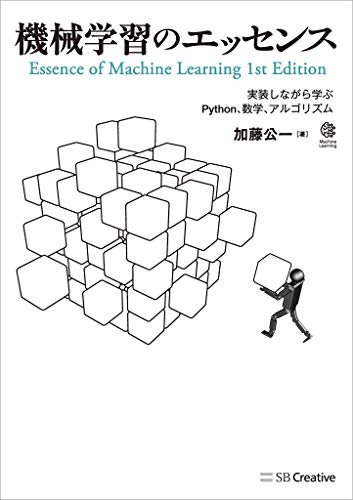
\includegraphics[scale=.2]{img/mlessence.jpeg}
\end{figure}
\begin{center}
  \url{https://bit.ly/mlessence}
\end{center}

\end{frame}
\begin{frame}[fragile]{今日の話}
  PythonのライブラリmathとNumPyについて
  \begin{itemize}
  \item mathってなに?NumPyってなに?
  \item mathとNumPyで何ができる?
  \item NumPyでできてmathでできないこと
  \item mathでできてNumPyでできないこと
  \item mathとNumPyの最近の進化
  \end{itemize}
\end{frame}
\begin{frame}[fragile]{この資料について}

  Latex + Beamerで書かれています。
  
  オープンソースで公開しています:\newline
  \url{https://github.com/hamukazu/stapy20230817}
\end{frame}
\begin{frame}[fragile]{mathとは?}
  オフィシャルサイトの説明:
  \begin{quote}
    This module provides access to the mathematical functions defined by the C standard.
  \end{quote}

  つまり、C言語の標準ライブラリmathで定義されている関数へのアクセスを提供する。

  {\tt math}はPythonの\emph{標準ライブラリ}(つまりPythonをインストールするとついてくる)
\end{frame}
\begin{frame}[fragile]{C言語のmathライブラリについて}
  
  C言語のmathライブラリの関数一覧はWikipedia参照:\newline
  {\tiny \url{https://en.wikipedia.org/wiki/C\_mathematical\_functions}}

  $\cos(\pi)$をCとPythonで計算してみる。
  
\begin{minipage}[t]{0.45 \textwidth}
\fontsize{6pt}{6pt}\selectfont    
\noindent  
C言語
\begin{verbatim}
#include <math.h>
#include <stdio.h>

int main()
{
  printf("%f\n", cos(M_PI));
}
\end{verbatim}
\end{minipage}
\begin{minipage}[t]{0.45 \textwidth}
\fontsize{6pt}{6pt}\selectfont    
\noindent  
Python
\begin{verbatim}
import math

print(math.cos(math.pi))
\end{verbatim}
\end{minipage}
\end{frame}
\begin{frame}[fragile]{C言語のmathとPythonのmathの差分}
\noindent
PythonにあってCにないものの例
\begin{itemize}
\item \verb|factorial|: 階乗($n!$)を計算
\item \verb|comb|: ${}_nC_k$を計算
\item \verb|perm|: ${}_nP_k$を計算
\item \verb|nlp|:(あとで説明します)
\end{itemize}
CにあってPythonにないものの例
\begin{itemize}
\item \verb|div|: 整数の割り算で商とあまりを同時に計算する(Pythonは\verb|divmod|が同じ機能)
\end{itemize}
以上を見ると、PythonのmathはCのmathの機能をできるだけカバーしようとしているが、独自で便利そうな関数も揃えている。
\end{frame}
\begin{frame}[fragile]{NumPyとは?}
  オフィシャルサイトのキャッチフレーズ:
  \begin{quote}
    The fundamental package for scientific computing with Python
  \end{quote}

  配列(array)とその操作に関する機能が特徴的(これは\verb|math|にはない機能)


  mathに含まれる関数はほぼNumPyにも含まれている。
  (例:sin, cos, exp, log, ...)
\end{frame}
\begin{frame}[fragile]{NumPyの配列の機能1:Vectorization}
配列に数値を作用させたときに自動的にベクトル化される  
\fontsize{10pt}{10pt}\selectfont    
\begin{verbatim}
>>> import numpy as np
>>> a = np.array([1,2,3])
>>> b = 5
>>> a + b
array([6, 7, 8])
\end{verbatim}
\end{frame}
\begin{frame}[fragile]{NumPyの配列の機能2:Broadcasting}
配列の演算が要素ごとの演算として解釈される
\fontsize{10pt}{10pt}\selectfont    
\begin{verbatim}
>>> import numpy as np
>>> a = np.array([1,2,3])
>>> b = np.array([4,5,6])
>>> a + b
array([5, 7, 9])
>>> a * b
array([ 4, 10, 18])
\end{verbatim}
\end{frame}
\begin{frame}[fragile]{NumPyの配列の機能3:Indexing}
  複数のインデクスを一度に指定して要素を取り出せる
\fontsize{10pt}{10pt}\selectfont    
\begin{verbatim}
>>> import numpy as np
>>> idx = np.array([1,3,5])
>>> a = np.array([10,20,30,40,50,60])
>>> a[idx]
array([20, 40, 60])
\end{verbatim}  
\end{frame}
\begin{frame}[fragile]{mathとNumPyの使い分け}
  例えば、expを計算するときに{\tt math.exp}と{\tt numpy.exp}のどちらを使うべきか。\vspace{1cm}


結論:どちらでもよいし、あまり悩む必要ない。

ただし、
  \begin{itemize}
  \item mathよりNumPyのほうが高機能なので、NumPyが当然動くことが期待されている環境では、何も考えずNumPyを使ったほうがよいかも(判断コスト、思考コストの低減)
  \item NumPyは外部モジュールであることに注意。依存ライブラリも含めてリリースする場合(例えば、Windowsのインストーラを作るとき、AWS Lambdaで使うとき)は、不必要なのにNumPyを含めるのは無駄にファイルが大きくなる。
  \end{itemize}
\end{frame}
\begin{frame}[fragile]{ここまでのまとめ}
  \begin{itemize}
  \item PythonのmathはC言語のmathをカバーすることを目標としている
  \item NumPyのほうがmathより高機能。特に配列機能が特徴的。
  \item mathはNumPyのほぼサブセットなので、NumPyが使えるような環境では、mathは使わなくてもほぼNumPyだけで完結できる。
  \end{itemize}
\end{frame}
\begin{frame}
  「mathはNumPyのほぼサブセット」

  
  「ほぼ」とは?
\end{frame}
\begin{frame}[fragile]{mathはほんとにnumpyのサブセット?}
mathにあってnumpyにない関数の一覧を取得してみる。
{\fontsize{6pt}{6pt}\selectfont    
\begin{verbatim}
>>> import mathp
>>> import numpy as np
>>> math_funcs = set([x for x in dir(math) if not x.startswith("_")])
>>> np_funcs = set([x for x in dir(np) if not x.startswith("_")])
>>> sorted(math_funcs - np_funcs)
['acos', 'acosh', 'asin', 'asinh', 'atan', 'atan2', 'atanh', 'comb', 
'dist', 'erf', 'erfc', 'factorial', 'fsum', 'gamma', 'isqrt', 'lgamma',
'perm', 'pow', 'tau', 'ulp']
\end{verbatim}
}
それなりにある!

以下(網羅的ではなく)中身を見ていきます。
\end{frame}
\begin{frame}[fragile]{逆三角関数と逆双曲線関数}
  $\sin$の逆関数(数学では$\sin^{-1}$と書いたり、$\arcsin$と書いたりする)は、mathでは\verb|asin|であり、numpyでは\verb|arcsin|である。

  
  $\sinh$の逆関数(数学では$\sinh^{-1}$と書いたり、arcsinhと書いたりする)は、mathでは\verb|asinh|であり、numpyでは\verb|arcsinh|である。

  以上、機能としては同じだが関数名が異なっている。
\end{frame}
\begin{frame}[fragile]{mathにあり、numpyにはないが、scipyにはあるもの}
  
  \verb|math.factorial| → \verb|scipy.special.factorial| ($n!$)
  
  \verb|math.comb| → \verb|scipy.special.comb| (${}_n C_k$)
  
  \verb|math.perm| → \verb|scipy.special.perm| (${}_n P_k$)

  \verb|math.gamma| → \verb|scipy.special.gamma| (ガンマ関数$\Gamma(x)$)
  
  \verb|math.lgamma| → \verb|scipy.special.loggamma| ($\log \Gamma(x)$)
\end{frame}
\begin{frame}[fragile]{{\tt math.ulp}}
  Pythonのドキュメントによる説明:
  {\small
  \begin{quote}
    \noindent math.ulp(x)
    
    \hspace{3mm}Return the value of the least significant bit of the float x:
  \end{quote}
}

least significant bitはunit in the last place(「最小変化単位」?日本語での一般的な訳はわからず)とも呼ばれ、その値を返す。
\end{frame}
\begin{frame}[fragile]{Unit in the last placeってなに?}
Wikipediaの解説:
\begin{figure}[!ht]
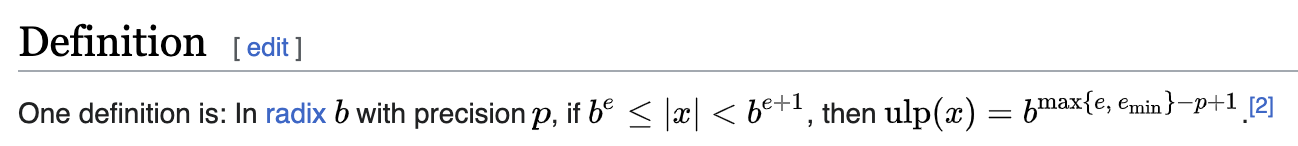
\includegraphics[scale=.4]{img/wikipedia-ulp.png}
\end{figure}
{\tiny \url{https://en.wikipedia.org/wiki/Unit\_in\_the\_last\_place}}

???

言い換えると、与えられた数に足すとコンピュータ内部表現としての数が変化するような数で最小のもの。

実行例:
{\fontsize{6pt}{6pt}\selectfont    
\begin{verbatim}
>>> import math
>>> math.ulp(1)
2.220446049250313e-16
>>> math.ulp(100)
1.4210854715202004e-14
>>> math.ulp(1e30)
140737488355328.0
\end{verbatim}
}
\end{frame}
\begin{frame}[fragile]{もっと詳しく知るために:浮動小数点数の内部表現}
  十進法の世界では、アボガドロ数:$6.02\times 10^{23}$のように、科学技術で使う数値は
  $\square.\square\square\square\square \times 10^{\square\square\square}$のようにされることが多い。

  特に仮数部の一の位がゼロにならないように調整する(例えば$6.02\times 10^{23} =
  0.602 \times 10^{24}$)
  
  二進法でも同様に$\square.\square\square\square\square_{(2)} \times 2^{\square\square\square}$で表す。

  二進法で仮数部の一の位がゼロでないように調整すると、一の位は1しかありえない。

\end{frame}
\begin{frame}[fragile]
  IEEE754では倍精度浮動小数点の内部表現を、符号1ビット、指数部11ビット、仮数部52ビットと規定している。
\begin{figure}[!ht]
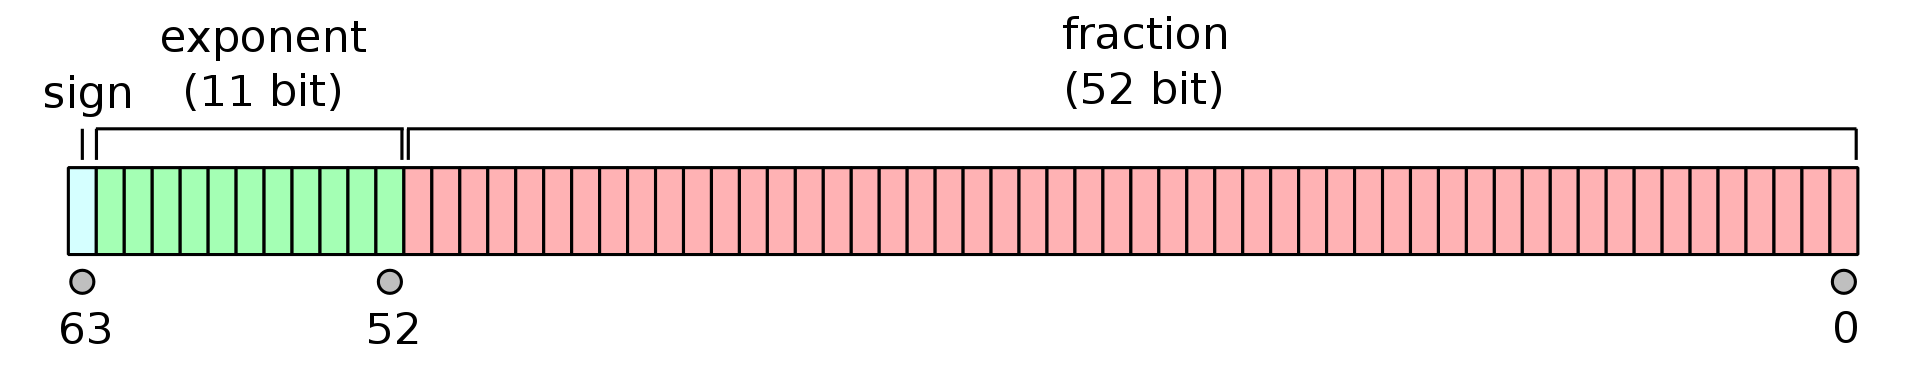
\includegraphics[scale=.1]{img/IEEE_754_Double_Floating_Point_Format.png}
\end{figure}

{\tiny 参照: \url{https://en.wikipedia.org/wiki/Double-precision\_floating-point\_format}}

符号は0:プラス、1:マイナス

指数部を符号なし11ビットとみなした数を$e$とすると、$e-1023$が指数となる(11ビットでは0から2047までの数を表せるが、0と2047は特別扱いとし、それ以外は$e-1023$を指数とする)

仮数は一の位が1として、残りの52ビットを仮数部で表現する。

\[ (-1)^\mathrm{sign} \times (1.b_{51} b_{50} \cdots b_{0})_{(2)} \times 2^{e-1023} \]
\end{frame}
\begin{frame}[fragile]
全ビットをゼロにしたものが0.0で、符号部を1にしてそれ以外を0にしたものが-0.0(0.0と-0.0は別)

{\tiny\tt
\begin{tabbing}
    -0.0 \=: (1 00000000000 0000000000000000000000000000000000000000000000000000)\kill
    0.0 \>: (0 00000000000 0000000000000000000000000000000000000000000000000000)\\
    -0.0 \>: (1 00000000000 0000000000000000000000000000000000000000000000000000)
  \end{tabbing}
}
指数部の全ビットを1にして仮数部の全ビットを0にしたのが$\pm\text{inf}$、仮数部に1があるのが{\tt nan}
{\tiny\tt
\begin{tabbing}
    0.0 \=: (1 00000000000 0000000000000000000000000000000000000000000000000000)\kill
    inf \>: (0 11111111111 0000000000000000000000000000000000000000000000000000)\\
    -inf \>: (1 11111111111 0000000000000000000000000000000000000000000000000000)\\
    nan \>: (0 11111111111 1000000000000000000000000000000000000000000000000000)
  \end{tabbing}
}


\end{frame}
\begin{frame}[fragile]
  例:アボガドロ数(の近似値)$6.02\times 10^{23}$はコンピュータ内部表現ではどうなっているか。
{\fontsize{6pt}{6pt}\selectfont
\begin{verbatim}
>>> import struct
>>> a = struct.pack(">d",6.02e23) 
>>> bit_expression = ("").join([("0"*7+bin(b)[2:])[-8:] for b in a])
>>> bit_expression
'0100010011011111110111101001111100010000101010001101001101100001'
>>> bit_expression[0], bit_expression[1:12], bit_expression[12:]
('0', '10001001101', '1111110111101001111100010000101010001101001101100001')
\end{verbatim}
}
指数部$11111101_{(2)}=1101_{(10)}$なので、指数は$1101-1023=78$となり、つまり、
\[
  6.02\times 10^{23} = 1.111111011110100\cdots_{(2)} \times 2^{78}
\]

ほんとかな?検算してみよう!
{\fontsize{6pt}{6pt}\selectfont    
\begin{verbatim}
>>> 0b1_1111110111101001111100010000101010001101001101100001/2**52 * 2**78
6.02e+23
\end{verbatim}
}
\end{frame}
\begin{frame}[fragile]{もう一度:Unit in the last placeってなに?}
  与えられた数の、符号を正にして、仮数部を$0.0\dots 001_{(2)}$(小数第52位が1でほかは0)だと思ったもの。

  
  例:
  $6.02\times 10^{23}$の内部表現は、
  {\tiny \[\mathtt{1.1111110111101001111100010000101010001101001101100001}_{(2)} \times 2^{1101-1023}\]}
  これのULPは
  {\tiny \[\mathtt{0.0000000000000000000000000000000000000000000000000001}_{(2)} \times 2^{1101-1023}\]}

  したがって、ULPより小さい数を足しても、コンピュータ内部では影響がない。
\end{frame}
\begin{frame}[fragile]
実行例
{\fontsize{8pt}{8pt}\selectfont
\begin{verbatim}
>>> import math
>>> a = 6.02e23
>>> math.ulp(a)
67108864.0
>>> a+1
6.02e+23
>>> a+1 == a
True
>>> a+100 == a
True
>>> a+10000 == a
True
>>> a+67108864.0 == a
False
\end{verbatim}
}
\end{frame}
\begin{frame}[fragile]
  以下mathとNumPyの最近のアップデートについて、数学的な注目点を説明します
  
  (変更点は大量にありますが、主に数学的な視点でピックアップします)
\end{frame}
\begin{frame}[fragile]{mathの新規追加関数}
  Python 3.11で次の関数が追加された。
  \begin{itemize}
  \item \verb|math.cbrt| : 立方根(三乗根)$\sqrt[3]{x}$を計算
  \item \verb|math.exp2| : 2のべき乗$2^x$を計算
  \end{itemize}
  これらは本当に必要?

  立方根は\verb|x**(1/3)|で計算できるし、2のベキは\verb|2**x|でいいのでは?

  →Cのmathにあるから追加すべきというのが理由の一つだが、他にも理由がある(後で説明)
\end{frame}
\begin{frame}[fragile]{ここでちょっと寄り道}
  \verb|**|と\verb|pow|と\verb|math.pow|の違いわかりますか?\vspace{7mm}

  
  \verb|pow|と\verb|math.pow|には第3引数があり、第3引数が与えられたときの\verb|pow|と\verb|math.pow|は同じ動作で、\verb|pow(n,k,m)|は引数がすべて整数であるときのみ有効で、$n^k \mod m$を意味する。

  第3引数が与えられないときの\verb|pow|と\verb|**|は同じで、\verb|math.pow|とは仕様が少し異なる。

  \verb|a|が負で\verb|b|が非整数の場合\verb|a**b|は複素数を返し、\verb|math.pow(a,b)|はエラーになる。

  (\verb|math.pow(a,b)|は値域が実数値になる指数関数に仕様を合わせている)
\end{frame}
\begin{frame}[fragile]
  実行例:
\fontsize{8pt}{8pt}\selectfont
\begin{verbatim}
>>> import math
>>> pow(2,3,5)
3
>>> (-1)**(1/2)
(6.123233995736766e-17+1j)
>>> pow(-1,1/2)
(6.123233995736766e-17+1j)
>>> math.pow(-1, 1/2)
Traceback (most recent call last):
  File "<stdin>", line 1, in <module>
ValueError: math domain error
\end{verbatim}
\end{frame}
\begin{frame}[fragile]{{\tt math.cbrt}の必要性}

    {\tiny 該当するGitHubでの議論: \url{https://github.com/python/cpython/issues/88523}}

  
  従来だと負の数の立方根を求めるのがとても不便。

  例:
  $\sqrt[3]{-8}=-2$だが...

{\fontsize{8pt}{8pt}\selectfont
\begin{verbatim}
>>> import math
>>> (-8)**(1/3)
(1.0000000000000002+1.7320508075688772j)
>>> math.pow(-8,1/3)
Traceback (most recent call last):
  File "<stdin>", line 1, in <module>
ValueError: math domain error
>>> math.cbrt(-8)
-2.0
\end{verbatim}
}
\end{frame}
\begin{frame}[fragile]
  参考:$a$が複素数、$b$が実数のときの\verb|a**b|の計算アルゴリズム\newline
  (=$a$が負で、$b$が非整数のときのアルゴリズム)

  まず、$a$の絶対値$\alpha$と偏角$\theta$を求める。つまり$a=\alpha (\cos\theta + i \sin\theta)$となる。
  
  あとは以下の式で計算:
  \[
    a^b = \alpha^b (\cos\theta + i \sin\theta)^b
    =\alpha^b (\cos b\theta + i \sin b\theta)
  \]

  例:
  $a=-8$, $b=1/3$のときは$\alpha=2,\,\theta=\pi$となるので\verb|a**b|は、
  \[
    8^{1/3} (\cos \pi/3 + i \sin \pi/3)
    =2\times\left( \frac{1}{2} + \frac{\sqrt{3}}{2}i \right)
    =1+\sqrt{3}i
  \]  
\end{frame}
\begin{frame}[fragile]{{\tt math.exp2}の必要性}
  
  {\tiny 該当するGitHubの議論:\url{https://github.com/python/cpython/issues/90075}}

  GitHubでは、\verb|math.pow|を使うより正確に計算できるという主張がなされているが、実験してみたところそうでもないらしい。

  Cのmathにあるからというのが唯一の理由?
\end{frame}
\begin{frame}[fragile]{{\tt math.pow}の仕様変更}
  
  Python 3.11から、\verb|math.pow(0.0,-inf)|と\verb|math.pow(-0.0,-inf)|は\verb|inf|を返すようになった(以前のバージョンではValueErrorになった)

  理由:IEEE 754でそう決められているから。

  ではなぜIEEEではそう決められているのか。
\end{frame}
\begin{frame}[fragile]
  仕様の確認:
  \verb|math.pow(a,b)|は値域が実数になる前提で考えている。
  \begin{itemize}
  \item \verb|a|が負のときは\verb|b|が整数のときのみ計算でき、それ以外はエラーになる。
  \item \verb|a|が正のときは\verb|b|は実数ならば何でもよい
  \end{itemize}

  では\verb|a|が0のときは?
  \begin{itemize}
  \item ${\tt b}\neq 0$かつ有限ならば、\verb|math.pow(0.0,b)=0.0|
  \item \verb|math.pow(0.0,0.0)=1.0| ($\lim_{a\to 0} a^0=1$だから)
  \item \verb|math.pow(0.0,inf)=0.0|
    ($0<a<1$のとき、$\lim_{b\to \infty} a^b=0$なので、$a\to +0$を考える)
  \item {[今回の仕様変更]} \verb|math.pow(0.0,-inf)=inf|
    ($0<a<1$のとき、$\lim_{b\to -\infty} a^b=\infty$なので、$a\to +0$を考える)
  \end{itemize}
\end{frame}
\begin{frame}[fragile]{{\tt numpy.percentile}, {\tt numpy.quantile}}
  NumPy ver 1.22.0で新しい引数\verb|method|が加えられた。

  {\tt numpy.percentile}と{\tt numpy.quantile}は、パーセントで指定するか割合($[0,1]$)で指定するかの違いだけで、他に違いはない。

  指定したパーセンタイルにぴったり数字が当てはまらないときは補間が必要だが、補間の仕方を\verb|method|で指定。
\end{frame}
\begin{frame}[fragile]
  methodのオプション一覧:
  {\tiny
  \begin{enumerate}
  \item ``inverted\_cdf''
  \item ``averaged\_inverted\_cdf''
  \item ``closest\_observation''
  \item ``interpolated\_inverted\_cdf''
  \item ``hazen''
  \item ``weibull''
  \item ``linear'' (default)
  \item ``median\_unbiased''
  \item ``normal\_unbiased''
  \end{enumerate}
  }
  これらそれぞれがどういう意味かというのは、NumPyのドキュメントには論文参照と書かれている。これらのオプションはR言語ですでに実装されているので、それを参考にしている。

  論文:R. J. Hyndman and Y. Fan, “Sample quantiles in statistical packages,” The American Statistician, 50(4), pp. 361-365, 1996
\end{frame}
\begin{frame}[fragile]{論文の概説}

  {\tiny R. J. Hyndman and Y. Fan, “Sample quantiles in statistical packages,” The American Statistician, 50(4), pp. 361-365, 1996}
  
  以下quantile(分位点)の方で話を進める。割合$p$に対するquantileを考える($p=0.5$のときが中央値で、$p=0.25$が第1四分位数、$p=0.75$が第3四分位数)。

  基本的なアイデア:ソートされたデータ$X_{(1)},X_{(2)},\ldots,X_{(n)}$があるとして、割合$p$に当たるインデックス$j$をピッタリと選べれば$X_{(j)}$が答えになり、そうでなければ、割合$p$に近い$j$について$X_{(j)}$と$X_{(j+1)}$で補間をとればよい。このインデックス$j$をどう取るかと、補間をどう計算するかの選択でいくつかのアルゴリズムが存在する。

  割合$p$に対するquantile $Q(p)$は以下の式で与えられる。

  $\displaystyle \frac{j-m}{n} \leq p < \frac{j-m+1}{n}$のとき
  $Q(p) = (1-\gamma) X_{(j)} + \gamma X_{(j+1)}$

  ただし、$\gamma$は$j=\lfloor pn+m \lfloor$と$g=pn+m-j$の関数であり、$m$は定数である。$\gamma$と$m$の選び方でアルゴリズムが決定される。
  
\end{frame}
\begin{frame}[fragile]
  
  具体例:
  
  データ[10,20,30,40,50,60,70,80,90]の第1四分位数($p=0.25$)は何でしょう?

  中間値が50である。

  「中間値を含んだ前半[10,20,30,40,50]の中間値30が第1四分位数である」(この場合$m=1-p$)という考え方もあるし...\newline
  「中間値を含まない前半[10,20,30,40]の中間値(の補間)25が第1四分位数である」(この場合$m=p$)という考え方もある。
  
\end{frame}
\begin{frame}[fragile]
  
  実行例:

{\fontsize{8pt}{8pt}\selectfont
\begin{verbatim}
>>> import numpy as np
>>> a = np.arange(10.,100,10)
>>> a
array([10., 20., 30., 40., 50., 60., 70., 80., 90.])
>>> np.quantile(a,0.25,method="linear")
30.0
>>> np.quantile(a,0.25,method="weibull")
25.0
>>> np.quantile(a,0.25,method="inverted_cdf")
30.0
>>> np.quantile(a,0.25,method="hazen")
27.5
\end{verbatim}
}
\end{frame}
\begin{frame}[fragile]{まとめ}
  \begin{itemize}
  \item sinなどの数学的関数は、NumPyが使える環境ならNumPyを使おう
  \item mathもNumPyも、いまでも進化しつづけている
  \item 浮動小数点数の内部構造について知っていると、数値計算関数の仕様の理解に役立つこともある
  \item 数学的計算をする関数の仕様は、数学の理論の観点から「自然な」仕様に決められていることが多い
  \item なぜそういう仕様になっているか知りたければ、GitHubのIssueでの議論を追えばよい
  \end{itemize}
\end{frame}
\end{document}
